% Warum manuell
% TODO: ggf. zusammenfassen
Viele Studien in der Literatur haben Klassifizierungsmethoden verwendet, um die Datensicherheit in der Cloud zu gewährleisten. Die vorgeschlagenen Lösungen lassen sich in zwei Klassen einteilen: die manuelle Klassifizierung, die vom Nutzer festgelegt wird, und die automatische Klassifizierung, bei der ein Algorithmus zum Einsatz kommt.

Die manuelle Datenklassifizierung ist trotz Fortschritte bei automatisierten Technologien eine gängige Methode. In einigen Fällen, wie bei der Klassifizierung von Informationen wie geistigem Eigentum oder Geschäftsgeheimnissen, bleibt die manuelle Klassifizierung erforderlich. Menschen sind in der Lage, leicht die Kategorien, Kontexte, Strukturen und Zustände der Daten ganzheitlich zu berücksichtigen. Außerdem kann die manuelle Klassifizierung für kleinere Unternehmen kostengünstig sein \cite{Divadari.2023}\cite{Alsuwaie.2021}.

% warum schwierig (aufwändig, fehlerbehaftet, Big Data)
Die manuelle Klassifizierung von Daten ist jedoch sehr anfällig für menschliche Fehler und Inkonsistenzen. Die Subjektivität der Menschen kann zu inkonsistenten Klassifizierungen führen, was die Genauigkeit und Zuverlässigkeit der Sicherheitsmaßnahmen beeinträchtigen kann. Zudem kann eine unzureichende Genauigkeit zu unvollständigen oder falschen Klassifizierungen führen. Im Normalfall werden Daten bei ihrer Erstellung klassifiziert, doch sie können sich im Laufe der Zeit ändern, wodurch die ursprüngliche Klassifizierung veraltet und nicht mehr richtig sein kann. Die manuelle Einordnung von großen Datenmengen kann sehr zeitaufwändig und arbeitsintensiv sein und ab einer bestimmten Größe nicht mehr manuell verarbeitet werden. Manuelle Prozesse können die Anpassungsfähigkeit und schnelle Reaktion auf sich ändernde Geschäftsanforderungen reduzieren \cite{Venhorst.2019}.

Aufgrund der wachsenden Datenmengen und der zunehmenden Komplexität der Informationssicherheitsanforderungen erscheint die automatisierte Datenklassifizierung häufig als effizientere Lösung, die eine genauere und konsistentere Identifizierung sensibler Daten ermöglicht.

% ###########################################
% warum automatisiert
Der Prozess, bei dem maschinelle Algorithmen und Technologien verwendet werden, um Daten automatisch zu identifizieren, zu kategorisieren und entsprechend ihres Sensitivität zu klassifizieren, wird als automatische Datenklassifizierung bezeichnet. Diese Methode verwendet maschinelles Lernen, Mustererkennung oder künstliche Intelligenz, um Daten zu analysieren und automatisch geeignete Klassifizierungen zuzuweisen.
Die aktuellen Techniken in der Data Leakage Prevention können allgemein in zwei Kategorien eingeteilt werden: inhaltsbasierte Analyse und kontextbasierte Analyse. Methoden, die auf dem Inhalt basieren, untersuchen den Inhalt von Daten anhand von Merkmalen sensibler Informationen wie regulären Ausdrücken und Datenfingerabdrücken. Inhaltsbasierte Methoden verwenden vorhersehbare Muster wie z.B. IP-Adressen oder E-Mail-Adressen, um sensible Daten zu erkennen. Kontextbasierte Techniken identifizieren vertrauliche Daten anhand von Merkmalen im Zusammenhanf mit den überwachten Daten. Der kontextbasierte Ansatz ist damit effektiver für vertrauliche Daten ohne vorhersehbare Muster \cite{Guo.2021}\cite{Gugelmann.2015}\cite{Kuzina.2023}. Um sensible Informationen umfassender und genauer zu extrahieren, sollten daher verschiedene Methoden angewendet werden. Die Tabelle \ref{t:methoden} zeigt die am häufigsten verwendeten Methoden in der Literatur. Die meisten kontexbasierten Ansätze kombinieren inhaltsbasierte und kontextbasierte Methoden, um die Vorteile beider Kategorien zu nutzen und die Genauigkeit der Klassifizierung zu verbessern.

%Tabelle mit content-based vs. context-based
\begin{table}[htbp]
    \normalsize
    \caption{Methoden der automatischen Datenklassifizierung. Quelle: eigene Darstellung.}
    \label{t:methoden}
    \begin{center}
        \begin{tabulary}{15cm}{|L|L|}
            \hline
            \textbf{Kategorie} & \textbf{Methode} \bigstrut  \\
            \hline
            \hline
            \multirow{5}{*}{inhaltsbasiert} & regelbasierte Methoden \bigstrut[t]     \\
            & Data Fingerprinting               \\
            & kNN              \\
            & Boosting \\
            & Clusteranalyse \\
            \hline
            \multirow{2}{*}{inhalts- und kontextbasiert} & CASSED  \bigstrut[t] \\
            & BERT-BiLSTM     \\
            \hline
        \end{tabulary}
    \end{center}
\end{table}

% ###########################################
\subsection{Klassifizierung mit manueller Definition}

% ###########################################
\paragraph{regelbasierte Methoden}
% rule-based/regular-matching/Dictionary
Eine einfache und häufig angewendete Technik zur automatischen Datenklassifizierung basiert auf einem Wörterbuch oder einer Regel, die im Wesentlichen den gegebenen Text mit einer Liste vordefinierter regulärer Ausdrücke und Schlüsselwörter abgleicht. Diese Methode verwendet vordefinierte Regeln und Bedingungen, um bestimmte Datentypen oder Muster automatisch zu identifizieren und zu klassifizieren. Diese Regeln können auf verschiedenen Merkmalen wie Schlüsselwörtern, Mustern, Dateiformaten oder spezifischen Attributen wie Datumsangaben basieren \cite{Ong.2017}.
Die Identifikation von Kreditkartennummern in Textdokumenten ist ein Beispiel für die Verwendung regelbasierter Methoden. Zur Erkennung kann ein regulärer Ausdruck verwendet werden, der die Zeichenfolge nach dem Muster einer Kreditkartennummer definiert. Muster in regulären Ausdrücken umfassen meistens normale Zeichen mit wörtlicher Bedeutung und Metazeichen, um ein Erkennungsmuster zu bilden \cite{Alneyadi.2016}.
Regeln können sich auch auf bestimmte Schlüsselwörter oder Phrasen beziehen, die auf personenbezogene Informationen wie \glqq Sozialversicherungsnummer\grqq \:oder \glqq vertraulich\grqq \:hinweisen können.
Der Vorteil regelbasierter Methoden liegt in ihrer klaren Struktur und der Möglichkeit, spezifische Anforderungen und Richtlinien der Organisation abzubilden. Sie ermöglichen eine präzise und konsistente Klassifizierung von Daten gemäß vordefinierten Sicherheitsstandards. Da die Klassifizierung auf klaren, vorher festgelegten Regeln basiert, ermöglichen regelbasierte Ansätze auch eine gewisse Transparenz und Nachvollziehbarkeit.
Jedoch können regelbasierte Methoden bei der Verarbeitung komplexer und sich verändernder Datenmuster weniger nützlich sein, da die Regeln schnell unpraktisch werden, wenn Datenformate, Kontext, Wortvariationen und Abkürzungen kombiniert werden müssen. Der Einsatz dieser Methode erfordert auch ein gut definiertes und gepflegtes Wörterbuch und Regelsatz. AAußerdem wird der semantische Kontext der Wörter bei einem reinen Textabgleich nicht berücksichtigt, was zu einer geringen Genauigkeit der Klassifizierung führen kann \cite{Ong.2017}.
Trotzdem bieten regelbasierte Ansätze eine grundlegende und robuste Methode zur Sicherstellung einer konsistenten Datenklassifizierung.

% ###########################################
\paragraph{Data Fingerprinting} \label{fingerprint}
Data Fingerprinting oder auch Document Fingerprinting erstellt eindeutige Fingerabdrücke für bestimmte Datenfragmente oder ganze Dateien. Diese Fingerabdrücke sind eindeutige Identifikatoren für die entsprechenden Daten und werden genutzt, um sensible Daten zu identifizieren und automatisch zu klassifizieren. Eindeutige Fingerabdrücke für Wörter, Sätze oder ganze Dateien werden mithilfe von Wortmustern aus regulären Ausdrücken oder vordefinierten Wörterbüchern erstellt und als Vorlage für sensible Daten verwendet. Diese Fingerabdrücke können dann verwendet werden, um Fingerabdrücke von nicht-klassifizierten Daten zu vergleichen und zu klassifizieren.
Häufig werden Hash-Funktionen wie MD5 oder SHA1 verwendet, um Datenfingerprints zu erstellen, die eine algorithmisch generierte Zeichenfolge fester Größe für die Daten darstellen. Die Hashes von zwei Dateien unterscheiden sich jedoch, sobald nur ein Zeichen verändert wurde \cite{Alneyadi.2016}. Ein weiterer Ansatz ist deshalb das \glqq Fuzzy-Hashing\grqq. Hierbei werden die Daten in Blöcken verarbeitet, wodurch die Hash-Ausgabe bei ähnlichen Daten größtenteils übereinstimmende Blöcke enthält. So kann die prozentuale Ähnlichkeit mithilfe einer mathematischen Vergleichsfunktion bestimmt werden \cite{Shu.2015}.

Sowohl im Speicher als auch bei Netzwerkübertragungen oder bei Verwendung kann das Data Fingerprinting sensible Daten erkennen. Der Fingerabdruck ist in manchen Fällen jedoch keine zuverlässige Methode. Die Klassifizierung funktioniert nicht, wenn die Daten verschlüsselt oder passwortgeschützt sind oder der Inhalt nicht eindeutig mit dem Fingerabdruck übereinstimmt. Außerdem ist es notwendig, dass die Vorlagen kontinuierlich aktualisiert werden und der Ansatz kann bei großen Datenmengen ressourcenintensiv sein.


% ###########################################
\subsection{Klassifizierung mit maschinellem Lernen}
% Ali Abdulsattar Jabbar, Wesam Sameer Bhaya 2023 – Security of private cloud using
% nur Text?
% Definition
% Datenaufbereitung
% wie wird Text in Algorithmen überhaupt dargestellt -> Vektoren
Die Datenklassifizierung ist eine Technik des maschinellen Lernens, mit der die Klasse der nicht klassifizierten Daten vorhergesagt wird. Dabei werden die Methoden in zwei Kategorien eingeteilt: überwachtes Lernen und unüberwachtes Lernen. Für überwachtes Lernen sind Testdaten mit bereits zugeteilten Klassen vordefiniert. So kann das Modell sein Ergebnis mit der Ziel-Klasse vergleichen und entsprechend von den Fehlern lernen. Beim unüberwachten Lernen sind keine Klassen definiert, sondern die Klassifizierung der Daten erfolgt automatisch. Ein unüberwachter Algorithmus sucht nach Mustern und Ähnlichkeiten zwischen den Elementen cite{Frochte.2018b}.

Für die meisten Methoden des maschinellen Lernens ist es erforderlich, dass die Daten vorab bereinigt oder vorbereitet werden. Die einzelnen Schritte können dabei je nach Methode variieren. Der Datensatz wird meistens von Stop-Wörtern bereinigt, die keinen oder nur wenig Kontext liefern wie bspw. 'und' oder 'der'. Klassische Methoden sind in der Textverarbeitung Stemming und Lemmatization. Beim Stemming werden die Worte der Eingabe auf ihren Wortstamm zurückgeführt, bei der Lemmatization werden ähnliche oder inhaltlich gleiche Begriffe vereinheitlicht.
Dadurch wird die grammatikalische Komplexität des Inputs reduziert und die Datenqualität optimiert. Für Methoden wie neuronale Netze müssen Eingabedaten zusätzlich noch in Token und Vektoren umgewandelt werden. Bei der Tokenization wird der Text ist einzelne Bestandteile, sogenannte Tokens aufgeteilt werden. Meistens sind das einzelne Worte. Die Tokens werden anschließend in Vektoren umgewandelt, die den jeweiligen Token im Modell repräsentiert. Für die Vektorisierung gibt es verschiedene Algorithmen, um Informationen wie inhaltlich ähnliche oder zusammenhängende Tokens zu behalten \cite{Kamath.2019}.


% ###########################################
\paragraph{k-NN}
% K-NN (k Nearest Neighbors)
Zardari, Jung et al. \cite{Zardari.2014} waren die ersten, die eine Methode aus dem maschinellen Lernen zur Datenklassifizierung verwendet haben, um im Cloud Computing die Datensicherheit zu verbessern. Sie verwendeten die k-Nearest Neighbor-Methode (k-NN), um Daten in der Cloud als sensibel und nicht-sensibel zu klassifizieren. k-NN ist eine Methode aus dem überwachten maschinellen Lernen und wird häufig zur Klassifizierung, Mustererkennung und Schätzung verwendet. Es handelt sich um einen sogenannten Instanz-basierten Algorithmus, der darauf basiert, dass ähnliche Dinge in der Regel nah beieinander liegen. Die k-NN-Methode verwendet die Nachbarn eines Datenpunkts, um Vorhersagen zu treffen oder Klassenzuweisungen zu machen. Der Algorithmus beginnt mit einem Datensatz, der aus Beispielen mit bekannten Klassen oder Werten besteht. Die Wahl des 'k' bestimmt die Anzahl der nächsten Nachbarn. Um die Ähnlichkeit zwischen den Datenpunkten zu bestimmen, wird ein Distanzmaß wie der euklidische Abstand oder die Manhattandistanz verwendet. Sie messen den Abstand zwischen den Merkmalsvektoren der Datenpunkte. Für einen gegebenen Datenpunkt werden die k nächsten Nachbarn basierend auf dem berechneten Distanzmaß aus dem Datensatz ausgewählt. Bei einer Klassifikation werden die Klassen der ausgewählten k Nachbarn betrachtet und die Mehrheitsklasse für den gegebenen Datenpunkt verwendet \cite{Frochte.2018b}.

In \cite{Zardari.2014} hat die Einteilung der Daten in zwei Klassen gut funktioniert. Doch die Wahl des passenden 'k' ist bei diesem Algorithmus entscheidend. Ein zu kleines 'k' kann dazu führen, dass potenziell passende Datenpunkte ausgeschlossen werden und ein zu großes 'k' führt zu einer zu groben Klassifizierung. Aufgrund der Verwendung aller Trainingsdaten ist zudem die Rechenkomplexität bei diesem Algorithmus hoch, da bei jeder Vorhersage der Abstand berechnet und die gesamten Trainingsdatendistanzen sortiert werden müssen. Außerdem ist die Mehrheitsentscheidung bei der Klassifizierung nicht immer die optimale Methode, da je nach Anzahl der Nachbarn die Abstände stark variieren können und trotzdem immer alle gewählten Nachbarn berücksichtigt werden.

% ###########################################
\paragraph{Boosting}
Ensemble Learning ist ein Begriff aus dem maschinellen Lernen und beschreibt das Zusammenschalten von mehreren Methoden, um das Modellergebnis zu verbessern. Der Ansatz beim Boosting ist, mehrere schwache Modelle zu einem starken Modell zusammenzusetzen \cite{Frochte.2018c}.
Kaur, Zandu \cite{Kaur.2016} schlagen für die Klassifizierung von sensiblen Daten eine neue Boosting-Architektur vor. Als Klassifikator wird eine Kombination aus dem Naive Bayes Klassifikator und AdaBoost verwendet. Der Naive Bayes Algorithmus ist eine Klassifizierungsmethode, die auf dem Bayes Theorem beruht. Die Grundlage ist die Annahme, dass das Auftreten eines Merkmals unabhängig mit dem Auftreten eines anderen Merkmals innerhalb der Klasse ist. Das Bayes Theorem ist eine Formel zur Berechnung der bedingten Wahrscheinlichkeit ${P(A|B)}$. Diese bedingte Wahrscheinlichkeit lässt sich mit der Formel \ref{e:naive-bayes} berechnen. Zur Klassifizierung eines Merkmals wird mit der Formel für jede Klasse berechnet, mit welcher Wahrscheinlichkeit das Merkmal zu dieser Klasse gehört. Gewählt wird schließlich die Zuordnung mit der höchsten Wahrscheinlichkeit \cite{Frochte.2018d}.

\begin{equation}
    \label{e:naive-bayes}
    P(A|B) = \frac{P(B|A) * P(A)}{P(B)}
\end{equation}

Im Ansatz von \cite{Kaur.2016} wird dieser Klassifikator mit AdaBoost, Abkürzung für adaptive Boosting, optimiert. AdaBoost kombiniert mehrere schwache Klassifikatoren zu einem starken Klassifikator. Dabei werden iterativ mehrere Klassifikatoren hinzugefügt und der Datensatz stetig neu gewichtet, damit sich der nächste Klassifikator auf die Fehler des vorherigen Klassifikators konzentriert \cite{Frochte.2018c}.

In der neuen Klassifikationsmethode von \cite{Kaur.2016} wird zuerst der Trainingsdatensatz in eine bestimmte Anzahl an Datensätzen aufgeteilt. Anschließend werden die einzelnen Teildatensätze schrittweise verarbeitet. Jeder Teildatensatz enthält eine Menge an Daten-Tupeln. Zu Beginn erhält jedes Tupel die gleiche Gewichtung. Dann wird das hybride Klassifizierungsmodell aus Naive Bayes und AdaBoost mit dem Teildatensatz trainiert. Anschließend werden bei den Tupeln die Gewichte aktualisiert, je nachdem ob sie richtig oder falsch klassifiziert wurden. Nach den Durchgängen aller Teildatensätze ergibt sich dadurch ein Set an Klassifikator-Modellen mit jeweiligen Gewichtungen, die in Kombination eine genaue Vorhersage für eine Klasse treffen.

Kaur, Zandu \cite{Kaur.2016} zeigten, dass ihre vorgeschlagene Methode mit 94,2529\% Genauigkeit deutlich besser klassifiziert als der k-NN-Algorithmus, der nur eine Genauigkeit von 51,7241\% hatte.

% ###########################################
\paragraph{Clusteranalyse}
% auf Basis von wenigen manuell klassifizierten Daten können Cluster gebildet werden
Die Clusteranalyse ist eine Datenanalysetechnik aus dem Bereich maschinellen Lernens. Clustering ist eine unüberwachte Lernmethode, die Muster in Eingabedaten ohne vordefinierte Zielwerte erkennt. Beim Clustering werden unsortierte Informationen auf der Grundlage von Ähnlichkeiten, Mustern und Unterschieden gruppiert, ohne dass die Daten zuvor trainiert wurden. Im Zusammenhang mit der Klassifizierung sensibler Daten wird die Clusteranalyse auf die Daten in einem Unternehmen angewendet. Die daraus resultierenden Cluster enthalten dann ähnliche Dokumente nach einer Ähnlichkeitsmetrik wie dem euklidischen Abstand oder der Kosinusähnlichkeit \cite{Suyal.2014}.
Um die Clusteranalyse als Klassifikator zu nutzen, müssen vor der Analyse relevante Merkmale oder Attribute definiert werden, um sensible Daten zu identifizieren. Anschließend können die Cluster anhand der Merkmale klassifiziert werden.

Zwei gängige Clustering-Methoden sind das hierarchische Clustering und das partitionierende Clustering. Hierarchisches Clustering wird in der Regel für dsa Clustering von Texten verwendet, wobei jedes Dokument auf der Grundlage seiner Ähnlichkeit schrittweise in einen vordefinierten Cluster zusammengeführt wird. Durch diesen Prozess entsteht eine Clusterhierarchie, die als Baumstruktur, das sogenannte Dendrogramm, dargestellt werden kann. Abbildung \ref{f:clustering_daten} zeigt einen Beispieldatensatz mit den Objekten a bis f. In diesem Datensatz liegen die Objekte b und c sowie d und e sehr nahe beieinander. Der Clustering-Algorithmus fasst dann nach und nach die Objekte mit dem geringsten Abstand zusammen,  gefolgt von den nächstgelegenen Objekten oder Clustern, bis der gesamte Datensatz gruppiert ist. So entsteht ein Baum wie in Abbildung \ref{f:clustering_baum}, bei dem die Blätter Cluster darstellen, die nur ein einzelnes Objekt aus dem Datensatz enthalten, und die Wurzel einen einzelnen Cluster, der alle Objekte enthält. Die Kanten zwischen den Knoten enthalten außerdem ein Attribut, das den Abstand zwischen den beiden Clustern angibt. Je nach gewünschter Anzahl von Clustern können die Cluster auf einer bestimmten Ebene des Baumes verwendet werden \cite{Suyal.2014}.
% TODO: Distanz Algorithmus im Detail darstellen?

\begin{figure}[htbp]
    \centering
    \begin{subfigure}[b]{0.47\linewidth}
        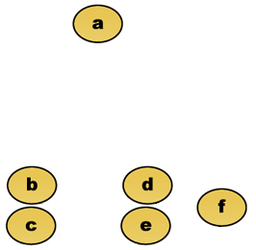
\includegraphics[width=\linewidth]{\figdir/clustering_daten}
        \caption{Datensatz. Quelle: In Anlehnung an \cite{Bonthu.2023}.}
        \label{f:clustering_daten}
    \end{subfigure}
    \hfill
    \begin{subfigure}[b]{0.47\linewidth}
        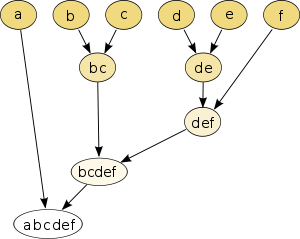
\includegraphics[width=\linewidth]{\figdir/clustering_dendrogramm}
        \caption{Dendrogramm. Quelle: In Anlehnung an \cite{Bonthu.2023}.}
        \label{f:clustering_baum}
    \end{subfigure}
\end{figure}

Aufgrund seiner Einfachheit und Flexibilität wird hierarchisches Clustering häufig verwendet und bietet den Vorteil, dass jede Art von Ähnlichkeitsmessung durchgeführt werden kann. Außerdem bietet dieses Verfahren eine detaillierte Darstellung der Clusterstruktur, wodurch unterschiedliche Granularitätsstufen von Clustern untersucht werden können.

% TODO: Partitionierende Clustering k-mean
Beim partitionierenden Clustering wird ein Datensatz in eine vorab definierte Anzahl von Clustern eingeteilt. Jeder Datenpunkt gehört zu einem bestimmten Cluster und das Ziel besteht darin, möglichst viele Datenpunkte in die Cluster zu verteilen und dabei die Ähnlichkeit zwischen den Clustern zu minimieren. DAs am weitesten verbreitete Verfahren ist der k-means-Algorithmus. Das 'k' steht für die Anzahl an zu definierenden Clustern und 'means' für den Mittelwert, also das Zentrum des Clusters. Zu Beginn muss die Anzahl der Cluster bestimmt werden. Dies kann sich z.B. daran orientieren, in welche Vertraulichkeitsstufen die Daten eingeteilt werden sollen. Anschließend werden für die Cluster initial jeweils zufällig ein Cluster-Mittelpunkt, auch Centroid genannt, gewählt. Dann wird für jeden Datenpunkt der Abstand zwischen dem Punkt und den Cluster Centroids berechnet. Der Punkt wird dem jeweiligen Cluster zugeordnet, welcher am nächsten ist und die Cluster sind initial befüllt. Nun folgen Schritte, die sich solange wiederholen, bis sich die Cluster nicht mehr ändern. Zuerst wird für jedes Cluster aus den Datenpunkten ein neuer Mittelwert bestimmt, der den neuen Centroid darstellt. Dann werden alle Datenpunkte anhand ihrer Distanzen zu den neuen Zentren neu zugeordnet \cite{Suyal.2014}.

Der k-mean Algorithmus ist beliebt, da er einfach ist, nur eine kleine Anzahl an Iterationen benötigt und parallel berechnet werden kann. Allerdings ist das Ergebnis des Algorithmus stark abhängig von der Wahl des 'k' und der initialen Cluster \cite{Suyal.2014}.


% ###########################################
\paragraph{Context-based Approach for Structured Sensitive Data Detection}
Kužina, Petric et al. \cite{Kuzina.2023} sahen eine große Herausforderung darin, sensible Daten in strukturierten Datenbanken zu klassifizieren. Das Problem besteht darin, die einzelnen Spalten einer Datenbanktabelle zu durchsuchen und zu bestimmten, ob sie sensible Daten enthalten und welche Arten sensibler Daten vorhanden sind. Dafür muss der Inhalt der Tabellen-Zelle interpretiert werden und der Kontext der umgebenden Zellen berücksichtigt werden. Bisherige Ansätze verwendeten dafür stark regelbasierte Methoden, deren Grenzen bei einer großen Menge an verschiedenen Datentypen schnell erreicht wurden. Außerdem können sie nur begrenzt Kontext und Semantik miteinbeziehen. Um dieses Problem zu lösen, entwickelten
Kužina, Petric et al. \cite{Kuzina.2023} eine neue Methode namens 'Context-based Approach for Structured Sensitive Data Detection' (CASSED). Dabei stellen sie einen Spaltenkontext durch die Kombination von Spaltenmetadaten und Zellwerten her, der in einen einzelnen Input-Vektor umgewandelt wird. Mit diesem Input-Vektor wird anschließend das BERT-Modell für die Klassifizierung verwendet.

BERT steht für 'Bidirectional Encoder Representations from Transformers' und ist ein von Google entwickeltes Open-Source Framework zur Erstellung von Transformer-basierten Natural-Language-Processing-Modellen. BERT ist darauf spezialisiert, kontextuelle Zusammenhänge und Beziehungen zwischen Wörtern zu erfassen. Transformer-basierte Modelle nutzen einen sogenannten Selbstaufmerksamkeitsmechanismus, indem die Beziehung eines Wortes mit jedem anderen Wort in einem Satz bestimmt wird. Außerdem enthalten sie mehrere Encoder- und Decoder Schichten, die einen Text lesen und versuchen, das nächste Wort vorherzusagen, sowie voll-vernetzte neuronale Netze. BERT nutzt Transformer, einen Aufmerksamkeitsmechanismus und nur Encoder-/Decoder-Schichten. BERT verarbeitet Texteingaben bidirektional, indem die Sequenzen sowohl von Anfang als auch vom Ende her analysiert werden, um ein besseres Verständnis für die kontextuellen Beziehungen der Wörter zu bekommen.

Im ersten Schritt erfolgt die Umwandlung der Spalten in Input-Vektoren. Dabei werden die Spaltenüberschrift zusammen mit mehreren Zellwerten derselben Spalte als Tokens dargestellt und durch Trennzeichen getrennt. In Abbildung \ref{f:input} ist eine Umwandlung einer Spalte in einen Input-Vektor dargestellt. Dabei wird die Spaltenüberschrift mit einem Punkt zur ersten Zelle getrennt, während die Zellen zueinander mit einem Komma getrennt werden. So wird dem Modell zusätzliche Informationen geliefert, dass diese Werte unterschiedlich behandelt werden sollten. BERT kann nur eine Anzahl von maximal 512 Tokens als Input-Vektor verarbeiten. Deshalb müssen größere Input-Vektoren noch aufgeteilt werden.

\begin{figure}[htbp]
    \centering
    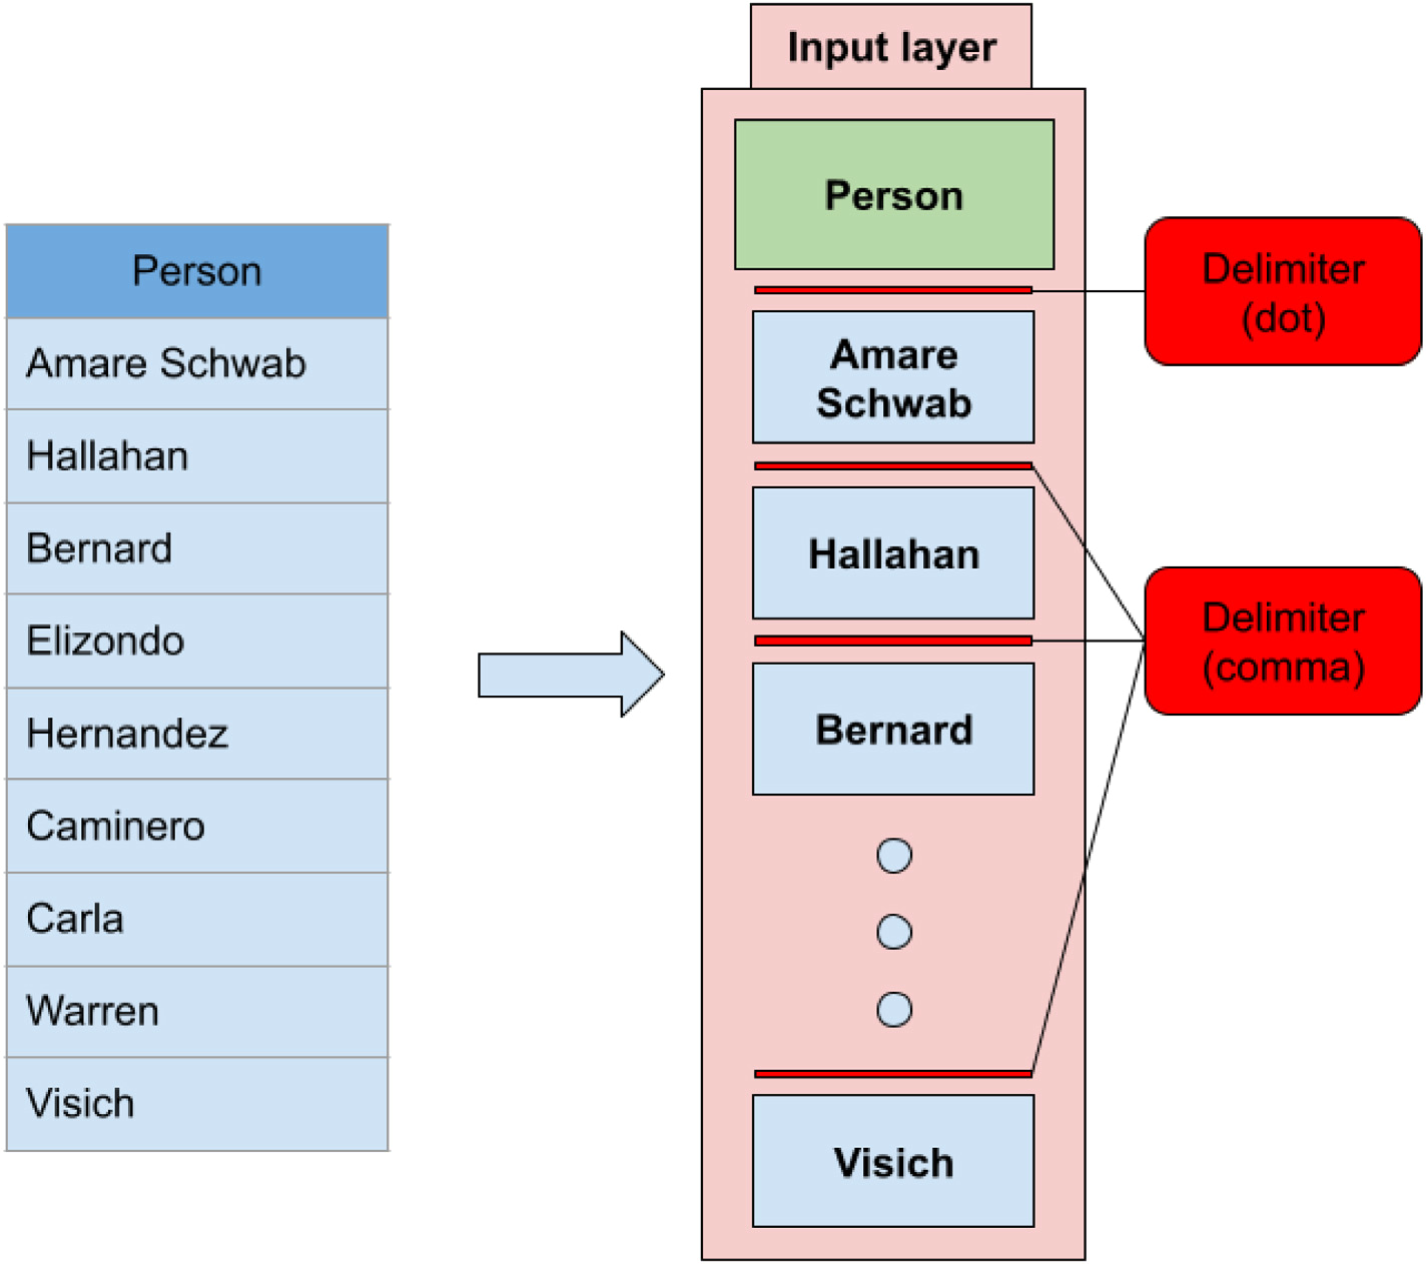
\includegraphics[width=0.8\linewidth]{\figdir/cassed_input.png}
    \caption{Beispiel einer Umwandlung einer Spalte in einen Input-Vektor. Quelle: \cite{Kuzina.2023}.}
    \label{f:input}
\end{figure}

Zur Klassifizierung erzeugt der Decoder von BERT für jede mögliche Klasse eine nicht normalisierte Vorhersage, die anschließend über alle Spaltenteile gemittelt wird, in die die Spalte aufgeteilt wurde. Auf diese Vorhersage-Werte wird eine Sigmoidfunktion angewendet, um normalisierte Wahrscheinlichkeiten für jede Klasse zu erzeugen.

Zusätzlich zum BERT-Modell enthält der CASSED-Ansatz eine regelbasierte Schicht, die strukturierte Formate wie E-Mails oder Sozialversicherungsnummern mittels regulären Audrücken klassifiziert. Außerdem wird ein Wörterbuch für bekannte sensible Daten oder Merkmale von Geschäftsgeheimnissen eingesetzt. Auch diese Schicht ermittelt für jede Klasse eine mögliche Wahrscheinlichkeit. Diese und die Wahrscheinlichkeiten der BERT-Schicht werden kombiniert zu einer Gesamt-Wahrscheinlichkeit pro Klasse. Anschließend werden die Klassen zugeteilt, deren Wahrscheinlichkeit einen bestimmten Schwellwert überschreiten. So ist es auch möglich, dass eine Spalte mehrere Klassen erhält. Abbildung \ref{f:cassed} stellt die Architektur des CASSED-Ansatzes dar.

\begin{figure}[htbp]
    \centering
    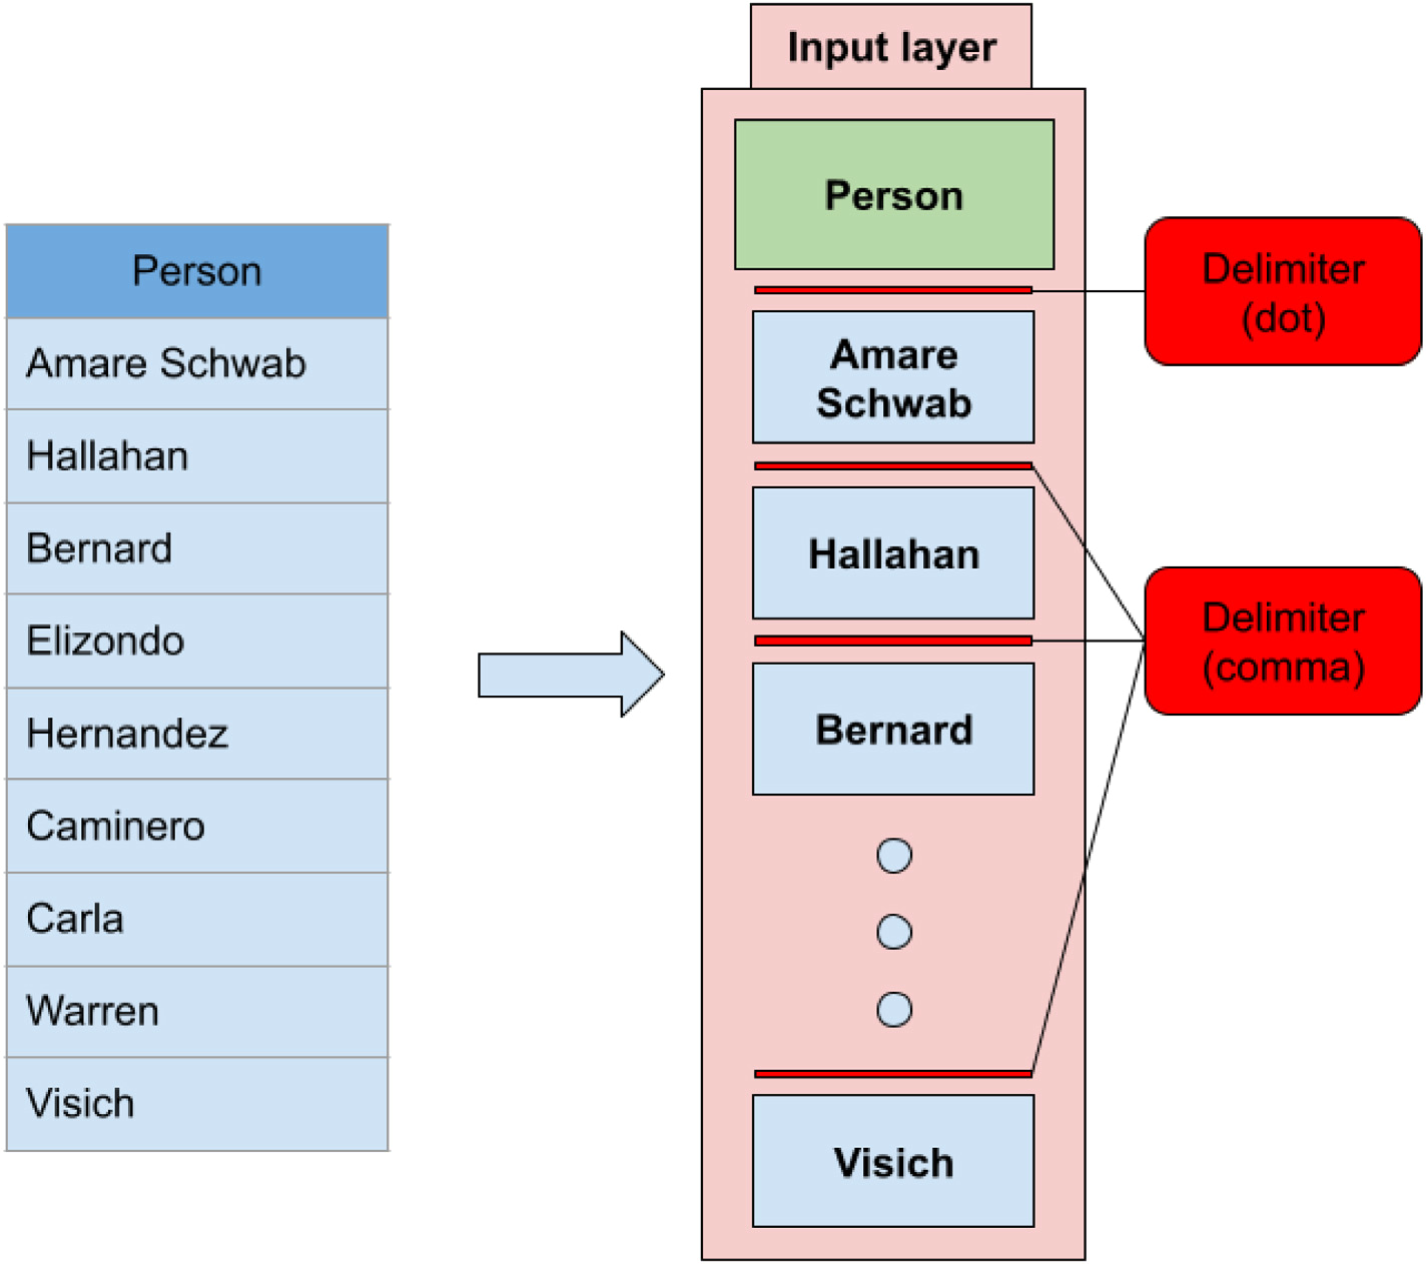
\includegraphics[width=0.8\linewidth]{\figdir/cassed_model.png}
    \caption{Überblick über die CASSED Methode. Quelle: \cite{Kuzina.2023}.}
    \label{f:cassed}
\end{figure}

Im Vergleich zu anderen kontextbasierten Klassifizierungsmethoden erzielt die CASSED Methode deutlich bessere Ergebnisse. Allein durch den reinen Einsatz von BERT schneidet das Modell besser ab und ist durch die regelbasierte Schicht sogar noch präziser.

Einen ähnlichen Ansatz verfolgen auch Guo, Liu et al. \cite{Guo.2021} mit ihrem Ansatz 'Exsense'. Auch sie verwenden zwei Schichten: eine inhaltsbasierte Analyse mit regulären Ausdrücken und eine kontextbasierte Analyse mit einem BERT-BiLSTM-Attention-Modell. Dabei wird das BERT-Modell kombiniert mit einem Bidirectional Long Short-Term Memory Modell (BiLSTM). BiLSTM ist ein rekurrentes neuronales Netzwerk, das für die Verarbeitung von sequenziellen Daten entwickelt wurde und gut darin, Abhängigkeiten in langen Sequenzen zu erfassen. Im BERT-BiLSTM-Modell wird die bidirektionale Kontextrepräsentation von BERT als Eingabe für das BiLSTM verwendet. Auch dieser Ansatz erzielte sehr gute Ergebnisse zur Klassifizierung von sensiblen Daten unter Berücksichtigung des Kontextes.


% ###########################################
% \paragraph{TF-IDF}
%'Term Frequency' und 'Inverse Document Frequency' (TF-IDF) ist eine häufiger verwendete Technik, bei der die Bedeutung eines Begriffs direkt proportional zur Häufigkeit des Auftretens des Begriffs in einem Dokument ist und umgekehrt proportional zur Häufigkeit des Auftretens des Begriffs im gesamten Dokument ist. Diese Technik wird häufig in verschiedenen Bereichen wie Data Mining oder Textklassifizierung eingesetzt.

% ###########################################
\subsection{Anwendung in der Cloud Security}
% wofür ist das dann gut
Wie in Kapitel \ref{dlp-kapitel} beschrieben, ist die Datenklassifikation ein wichtiger Bereich in DLP-Systemen, da die verschiedenen Sicherheitsmaßnahmen und Techniken auf der Kenntnis über die Sicherheitsstufen der Daten basieren. Deshalb bieten viele DLP-Systeme Funktionen zur automatischen Erkennung und Klassifizierung von sensiblen Daten.
Google Cloud Data Loss Prevention ist ein vollständig verwalteter Dienst, der es Unternehmen ermöglicht, sensible Daten in Cloud- und lokalen Umgebungen zu erkennen, zu klassifizieren und zu schützen. Der Dienst nutzt dabei maschinelles Lernen und Mustervergleichstechniken, um bis zu 150 verschiedenen Datentypen zu identifizieren und sie anhand dessen zu klassifizieren. Durch die Einstufung der Daten in verschiedene Datentypen und Klassen können in dem Cloud-DLP-System dann verschiedene Schutzmaßnahmen definiert werden \cite{GoogleCloud.30.11.2023}.

Das Software-Produkt Digital Guardian Cloud Data Protection ist ein Cloud-DLP-System des Anbieters Fortra. Das System besteht aus vielen verschiedenen Modulen, wobei eines davon Datenklassifizierung ist. Das Modul identifiziert und klassifiziert sensible Daten und hängen ihnen verschiedene Sicherheitsstufen-Labels an. Dabei verwendet das Modul automatische inhalts- und kontextbasierte Klassifizierung, doch auch eine manuelle Klassifizierung durch den Benutzer ist möglich. Das Cloud-DLP-System von Fortra ist dabei mit allen gängigen Cloud-Plattform-Anbietern kompatibel \cite{DigitalGuardian.30.11.2023}.

Die Klassifizierung und das entsprechende Markieren der Daten dient in Cloud-DLP-Systemen anschließend dazu, geeignete Schutzmaßnahmen zu definieren. Im Folgenden werden verschiedene Techniken beschrieben, die eine versehentliche Offenlegung von sensiblen Daten verhindern.

% Wasserzeichen
Eine der ersten Techniken zum Schutz von sensiblen Daten ist die Wasserzeichen-Methode. Dabei werden spezifische Identifikationsmerkmale oder Muster durch einen Algorithmus in Daten eingebettet, um die Quelle oder den Eigentümer zu kennzeichnen. Wasserzeichen dienen dazu, den Ursprung von Daten zu verfolgen und zu überwachen, um unbefugte Verbreitung oder Weitergabe zu erkennen. Systeme können anhand der eingebetteten Wasserzeichen erkennen, wenn Daten ohne Berechtigung weitergegeben oder veröffentlicht werden und Maßnahmen ergreifen. So können mithilfe von Wasserzeichen Datenlecks und -manipulationen erkannt und verhindert werden \cite{Naik.2019}.

%Blacklisting, Whitelisting
Eine weit verbreitete Methode in DLP-Systemen ist das Blacklisting oder Whitelisting. Dabei wird ein Modell verwendet, das aus Regeln besteht, die Muster böswilliger Aktivitäten oder markierte sensible Daten definieren, die das Unternehmensnetzwerk nicht verlassen dürfen. Beim Whitelisting wird definiert, welche Daten geteilt werden dürfen, beim Blacklisting werden die Daten und Muster definiert, die nicht geteilt werden dürfen. So kann ein DLP-System anhand dieser Regeln und Listen Transaktionen blockieren und so eine versehentliche Offenlegung von sensiblen Daten verhindern. Allerdings ist es für böswillige Insider oft leicht, eine Blacklisting-basierte Erkennung zu umgehen, da je nach Berechtigungen die Regeln und Listen bekannt sind \cite{Costante.2016}.

% Verschlüsselung
Die Kryptografie ist die am häufigsten verwendete Technik im Datenschutz. Sie wandelt Informationen von einem lesbaren Format in ein verschlüsseltes Format um. Je nach Sicherheitsstufe der Daten können unterschiedliche Verschlüsselungsalgorithmen und kryptografische Funktionen zum Einsatz kommen \cite{HerreraMontano.2022}. Dabei ist es nicht sinnvoll, einfach alle vorhandenen Daten verschlüsselt zu speichern oder zu übertragen. Insbesondere bei großen Datenmengen kann das schnell zu Performance-Problemen führen. Die Verschlüsselung von Daten erfordert Rechenressourcen und erhöhten Speicherbedarf. Deshalb wird meistens nur nach Bedarf verschlüsselt \cite{Arki.2023}.
Zardari, Jung et al. \cite{Zardari.2014} kategorisieren in ihrem vorgeschlagenen Modell Daten nach sensibel und nicht-sensibel. Nicht-sensible Daten werden direkt im Cloud-Speicher gespeichert, sensible Daten werden vorher mit dem RSA-Algorithmus verschlüsselt.

% Hashing
Das Fingerprinting-Verfahren, das in \ref{fingerprint} zur automatischen Klassifizierung beschrieben wurde, kann auch als Schutzmaßnahme dienen. Mit einem Vergleich von Datei- oder Daten-Hashes kann der ausgehende Datenverkehr überwacht werden. Ein DLP-System gleicht dabei die Hashes der Daten im Datenverkehr mit denen der als sensibel markierten Daten ab und kann so bei Übereinstimmung ein Datenleck erkennen und verhindern. Auch hier ist die Wahl des Hashing-Verfahrens relevant, wie verlässlich auch veränderte Daten noch erkannt werden \cite{HerreraMontano.2022}.

% Cloud Shredder
Zhang, Jing et al. \cite{Zhang.2011} stellen eine Methode vor, um die versehentliche Offenlegung von sensiblen Daten zu verhindern, selbst wenn bspw. ein ungeschützter Laptop verloren geht. Der Ansatz namens 'Cloud Shredder' sieht vor, dass vertrauliche Dateien geschreddert, also in Stücke geteilt wird, und ein Teil auf dem physischen Gerät und ein Teil im Cloud-Speicher gespeichert wird. Nur, wenn man Zugriff auf beide Bereiche hat, kann man die sensiblen Dateien lesen oder verarbeiten.

% DocGuard
Ein weiterer Ansatz namens 'DocGuard' wurde von Gui, Puzis et al. in \cite{Guri.2019} vorgestellt. Die Idee besteht darin, dass bereits vorhandene Antiviren-Software durchgesickerte Daten identifizieren und den Zugriff blockieren. Das funktioniert, indem DocGuard bei sensiblen Daten eine versteckte Signatur einer bekannten Schadsoftware einfügt. Wenn diese Daten das Unternehmensnetzwerk verlassen, erkennt eine Antiviren-Software die schadhafte Signatur als Bedrohung und greift ein.

% BrowserFlow
In Unternehmen werden externe Cloud-Dienste wie Google Docs immer mehr genutzt. Dabei können Benutzer schnell gegen unternehmensinterne Daten-Richtlinien verstoßen. Schnell sind sensible Daten aus einem geschützten Cloud-Dokument in ein ungeschütztes Cloud-Dokument kopiert und damit offengelegt. Papagiannis, Watcharapichat et al. \cite{Papagiannis.2016} schlagen als Lösung für dieses Problem ihren Ansatz namens 'BrowserFlow' vor. BrowserFlow ist eine browserbasierte Middleware, die Datenflüsse verfolgt, indem sie die Ähnlichkeit zwischen Textfragmenten erkennt. Anhand von gekennzeichneten Daten können so nicht autorisierte Datenflüsse identifiziert und verhindert werden.
